% Options for packages loaded elsewhere
\PassOptionsToPackage{unicode}{hyperref}
\PassOptionsToPackage{hyphens}{url}

\documentclass[referee,usenatbib]{biom}

\setlength{\paperwidth}{8.5in}
\setlength{\paperheight}{11in}

\usepackage{xr}
\makeatletter
\newcommand*{\addFileDependency}[1]{% argument=file name and extension
  \typeout{(#1)}
  \@addtofilelist{#1}
  \IfFileExists{#1}{}{\typeout{No file #1.}}
}
\makeatother

\newcommand*{\myexternaldocument}[1]{%
    \externaldocument{#1}%
    \addFileDependency{#1.tex}%
    \addFileDependency{#1.aux}%
}

\myexternaldocument{BSET_appendix}

\newcommand{\argmin}{\mathop{\rm arg\min}}
\newcommand{\argmax}{\mathop{\rm arg\max}}

\usepackage[dvipsnames,svgnames,x11names]{xcolor}
\usepackage{graphicx,verbatim,array,multicol,lscape,mathrsfs,color,enumitem}
\usepackage{amsmath,amsfonts,epsfig,fancybox,soul,float,subcaption,booktabs,pdflscape}
\usepackage{algorithm,algorithmicx,algpseudocode}
\usepackage[hidelinks]{hyperref}
\def\bW{{\bf W}}
\def\bZ{{\bf Z}}
\def\bL{{\bf L}}
\def\bw{{\bf w}}
\def\supone{^{(1)}}
\def\supzero{^{(0)}}
\def\supg{^{(g)}}
\def\transpose{{\sf \scriptscriptstyle{T}}}
\def\bU{{\bf U}}
\def\bUhat{{\widehat \bU}}
\def\trans{^{\transpose}}
\def\var{\text{Var}}
\def\bbeta{\boldsymbol{\beta}}
\def\bomega{\boldsymbol{\omega}}
\def\bPi{\boldsymbol{\Pi}}
\def\calt{\mathcal{T}}
\def\bSigma{\boldsymbol{\Sigma}}
\def\bmu{\boldsymbol{\mu}}
\newtheorem{proposition}{Proposition}

\usepackage{bbm}
\usepackage{multirow}

\newcommand{\E}{\mathbb{E}}
\newcommand{\N}{\mathbb{N}}
\newcommand{\R}{\mathbb{R}}
\newcommand{\Prob}{\mathbb{P}}
\newcommand{\iid}{\overset{\text{\footnotesize i.i.d.}}{\sim}}
\newcommand{\indepsim}{\overset{\text{ind.}}{\sim}}
\newcommand{\indep}{\perp \!\!\! \perp}
\newcommand{\one}{\mathbbm{1}}

\allowdisplaybreaks

\providecommand{\tightlist}{%
  \setlength{\itemsep}{0pt}\setlength{\parskip}{0pt}}
\usepackage{longtable,array}
\usepackage{calc}
\usepackage{etoolbox}
\makeatletter
\patchcmd\longtable{\par}{\if@noskipsec\mbox{}\fi\par}{}{}
\makeatother
\IfFileExists{footnotehyper.sty}{\usepackage{footnotehyper}}{\usepackage{footnote}}
\makesavenoteenv{longtable}
\graphicspath{{figures/}}
\makeatletter
\def\maxwidth{\ifdim\Gin@nat@width>\linewidth\linewidth\else\Gin@nat@width\fi}
\def\maxheight{\ifdim\Gin@nat@height>\textheight\textheight\else\Gin@nat@height\fi}
\makeatother

\begin{document}

\setlength\parindent{15pt}

\title{A Bayesian Critique of Rank-Based Methods for Surrogate Marker Evaluation}

\author{Pietro Carlotti \\ Department of Statistics and Data Sciences, University of Texas at Austin \\ pietro.carlotti@utexas.edu \and Layla Parast \\ Department of Statistics and Data Sciences, University of Texas at Austin \\ parast@austin.utexas.edu}

\begin{abstract}
Surrogate markers are often employed in clinical trials to replace primary outcomes that may be difficult, expensive, or time-consuming to measure directly. These markers can accelerate the evaluation of new treatments, provided they reliably capture the causal relationship between treatment and true clinical benefit. \citet{parast2024rank} recently proposed a rank-based approach for evaluating surrogate markers, characterized by its nonparametric nature and minimal assumptions. While this method is useful in small-sample model-agnostic settings, it has several limitations, including a lack of clear causal interpretation, low statistical power, and insufficient robustness to different data-generating mechanisms. In this paper, we propose a Bayesian approach that addresses these shortcomings by focusing on causal treatment effect estimands and, in doing so, improves power through covariate adjustment. To demonstrate the advantages of our proposed method, we conduct a comprehensive evaluation using both a simulation study, designed to highlight gains in accuracy and statistical power, and an application to a real clinical trial dataset.
\end{abstract}

\begin{keywords}
Bayesian Inference; Surrogate Markers; Clinical Trials; Causal Inference.
\end{keywords}

\maketitle


\section{Introduction}\label{sec:introduction}

Surrogate markers are often employed in clinical trials to replace primary outcomes that may be difficult, costly, or time-consuming to measure \citep{annurev:/content/journals/10.1146/annurev-statistics-032921-035359}. These markers can accelerate the evaluation of promising new treatments, provided that they reliably capture the causal relationship between treatment and true clinical benefit.
%For example, \citet{lavine2010treatment} conducted a clinical trial evaluating various treatments for children with nonalcoholic fatty liver disease, in which the primary outcome, a measure of liver function, was obtained via liver biopsy, a very invasive procedure. Instead, this study examined treatment effectiveness using a surrogate marker, change in alanine aminotransferase (ALT), a blood-based enzyme that reflects liver function, thus substantially reducing patient burden.
Notably, in the United States, the Food and Drug Administration's (FDA) Accelerated Approval Program, established in 1992, allows new treatments to receive early approval based on demonstrated effects on surrogate markers, and many drugs have been approved, and continue to be approved, through this pathway over time \citep{FDA_AcceleratedApprovalProgram2024,FDA_approved}.

A valid surrogate can substantially reduce trial burden, duration, and cost while still providing meaningful information about treatment efficacy, thereby enabling more timely access to effective treatments. However, establishing \textit{surrogate validity} is a challenging statistical problem, requiring methods that are both robust and interpretable. On this account, surrogate evaluation has been an active area of research, particularly because the FDA does not provide a formal statistical definition of a valid surrogate. A recent review by \citet{elliott2023surrogate} summarizes the state of proposed and currently used methods, including the proportion of treatment effect explained (PTE) framework \citep{freedman1992statistical,wang2002measure,parast2015robust,parast2025surrogate}, the principal stratification framework \citep{frangakis2002principal,gilbert2008evaluating}, and the meta-analytic framework \citep{buyse1998criteria,burzykowski2005evaluation,huang2011comparing}.

Unfortunately, these methods often perform poorly in small trials, especially when using robust techniques such as kernel-based estimation within the PTE framework. To address this, \citet{parast2024rank} proposed a rank-based approach for evaluating surrogate markers in such settings. Despite its attractive nonparametric nature and minimal assumptions, this method has notable limitations, including unclear causal interpretation for its target estimands, low power, and limited robustness across data-generating mechanisms.

In this paper, we improve upon this existing approach by proposing an imputation-based Bayesian alternative that extends the rank-based framework of \citet{parast2024rank}. Our approach is grounded in Bayesian causal inference, which treats unobserved potential outcomes as latent variables and samples them from predictive distributions \citep{li2023bayesian}. By using this perspective, our method not only provides a causal interpretation but also allows for covariate adjustment, improved efficiency, and a flexible framework for inference.

The rest of this work is organized as follows. In Section~\ref{sec:methods}, we review the existing rank-based approach for surrogate evaluation, outline its limitations, and highlight how the choice of treatment effect estimands can affect conclusions about surrogate validity. In Section~\ref{sec:bayesian_approach}, we present our Bayesian methodology, including two parametric models and a new criterion for the surrogate validation threshold. In Section~\ref{sec:simulation_study}, we present a simulation study comparing our proposed method with the existing approach, and in Section~\ref{sec:real_data_application}, we apply our method to a clinical trial dataset. Finally, Section~\ref{sec:discussion} discusses potential future extensions.

\section{Methods}\label{sec:methods}

\subsection{Notation}\label{subsec:notation}

Let \(Y\) denote the primary outcome and \(S\) the surrogate marker. Let \(Z \in \{0,1\}\) be the treatment indicator, assigned at random, where \(Z=1\) indicates treatment and \(Z=0\) control. Without loss of generality, assume higher values of \(Y\) and \(S\) correspond to greater clinical benefit. We adopt the potential outcomes framework to define causal effects \citep{rubin1974estimating}. For each unit \(i \in \{1,\ldots,n\}\), let \(Y_{gi}\) and \(S_{gi}\) denote the potential outcomes for the primary and surrogate under treatment \(g \in \{0,1\}\). The potential outcomes for unit \(i\) are
\[
  P_{i} = (Y_{0i}, Y_{1i}, S_{0i}, S_{1i})^{\top}.
\]
We assume that for each unit \(i\), the vector of potential outcomes \(P_i\) is independently drawn from a joint distribution \(F_i\), which may differ across units, and that the treatment assignment \(Z_i\) is independently drawn from a Bernoulli distribution, with \(Z_i \indep P_i\) by design. Only the potential outcomes corresponding to the observed treatment assignment are observed. That is, each unit \(i\) contributes \(P_{1i} = (Y_{1i}, S_{1i})^{\top}\) when \(Z_i = 1\), and \(P_{0i} = (Y_{0i}, S_{0i})^{\top}\) when \(Z_i = 0\). The hierarchical process that generates the data is summarized as follows:
\begin{equation}
  \label{eq:data_generating_process}
  \begin{aligned}
    (Y_{i}, S_{i})^{\top} &=
    \begin{cases}
      P_{1i}, & \text{if } Z_{i} = 1, \\
      P_{0i}, & \text{if } Z_{i} = 0,
    \end{cases} \quad i = 1, \ldots, n, \\
    P_i &\overset{\text{\footnotesize ind.}}{\sim} F_i, \quad i = 1, \ldots, n, \\
    Z_{i} &\iid \text{Bernoulli}(p), \quad i = 1, \ldots, n,
  \end{aligned}
\end{equation}
where \(p\) is the known treatment assignment probability (e.g., \(p = 0.5\) for a balanced trial). Finally, we denote the vector of observed data for unit \(i\) as \(D_i = (Y_i, S_i, Z_i)^{\top}\) or \(D_i = (Y_i, S_i, Z_i, X_i)^{\top}\), when covariates are available.

In the next section, we describe the existing rank-based approach for evaluating a surrogate marker and call attention to its key limitations.

\subsection{Existing Frequentist Rank-Based Approach}\label{subsec:frequentist_approach}

The main idea of \citet{parast2024rank} is that if \(S\) is a valid surrogate for \(Y\), then the treatment \(Z\) should have comparable effects on both, on a probabilistic scale that is invariant to differences in the measurement units of \(Y\) and \(S\). Their method focuses on small-sample settings, where nonparametric kernel methods are infeasible and parametric models are difficult to validate. Motivated by this, they used the following probabilistic index
\begin{equation}
  \label{eq:U_definition}
  U_{Y} = \Prob(Y_{1i} > Y_{0j}) + \frac{1}{2} \Prob(Y_{1i} = Y_{0j}),
\end{equation}
as a measure of the treatment effect on the primary outcome \(Y\), where \(i\) and \(j\) index two different units. This quantity is often referred to as the Mann-Whitney parameter \citep{mann1947test, thas2012probabilistic, hoeffding1992class, buyse2010generalized}, as it is the estimand targeted by the corresponding hypothesis test. In this work, we restrict our attention to continuous outcomes, thereby excluding ties in Equation~\eqref{eq:U_definition}. Therefore, a positive treatment effect on \(Y\) is concluded if \(U_{Y} > 0.5\). The same reasoning applies to the surrogate \(S\), with \(U_{S}\) defined analogously. The discrepancy in treatment effects is then measured by their difference \(\delta = U_{Y} - U_{S}\). Based on this definition, \citet{parast2024rank} propose that, if \(S\) is a valid surrogate for \(Y\), \(\delta\) should be small, leading to the following hypothesis test
\begin{equation}
  \label{eq:hypothesis_test_delta}
  \begin{cases}
    H_{0}: \delta \geq \varepsilon, \\
    H_{1}: \delta < \varepsilon,
  \end{cases}
\end{equation}
where \(\varepsilon\) is a pre-specified threshold for surrogate validation.

To estimate the parameter of interest \(\delta\), \citet{parast2024rank} compute \(\widehat{U}_{Y}\) and \(\widehat{U}_{S}\) using plug-in estimators, commonly known as the Mann--Whitney U-statistics:
\begin{equation}
  \label{eq:U_estimator}
  \begin{aligned}
    \widehat{U}_{Y} & = \frac{1}{n_{1} n_{0}} \sum^{n_{1}}_{i = 1} \sum^{n_{0}}_{j = 1} \one(Y_{i} > Y_{j}), \\
    \widehat{U}_{S} & = \frac{1}{n_{1} n_{0}} \sum^{n_{1}}_{i = 1} \sum^{n_{0}}_{j = 1} \one(S_{i} > S_{j}),
  \end{aligned}
\end{equation}
where \(n_{1}\) and \(n_{0}\) are the treated and control sample sizes, and then estimate \(\delta\) by \(\widehat{\delta} = \widehat{U}_{Y} - \widehat{U}_{S}\). A confidence interval for \(\delta\) follows from the central limit theorem for U-statistics and closed-form variance estimators for linear combinations of U-statistics. \citet{parast2024rank} conclude that \(S\) is valid if the upper bound of this interval is less than the pre-specified threshold \(\varepsilon\).

\subsection{Limitations of the Existing Approach}\label{subsec:limitations}

The nonparametric approach of \citet{parast2024rank} suffers from several notable limitations. Firstly, it is worth questioning whether the treatment effect quantities considered truly capture the causal targets. In the causal inference literature, rank-based statistics have in fact been criticized for lacking a clear causal interpretation \citep{imbens2015causal}. For example, the Mann--Whitney test assesses whether two variables are equal in distribution, but this condition is not necessarily informative about causal effects. To illustrate this point, note that since \(U_{Y}\) represents the probability that a randomly selected treated unit has a higher Y than an independently selected control, it captures global distributional differences between groups, rather than a directly interpretable causal effect. This motivates the consideration of alternative estimands that more directly target causal effects, such as
\begin{equation}
  V_{Y} = \Prob(Y_{1i} > Y_{0i}),
\end{equation}
which represents the probability that a randomly selected unit has a better outcome \(Y\) under treatment than under control. If we define \(V_{S}\) analogously for the surrogate \(S\), then we can measure the discrepancy in treatment effects via \(\theta = V_{Y} - V_{S}\). Notably, \(U_{Y}\) and \(U_{S}\) are not equivalent to \(V_{Y}\) and \(V_{S}\), as discussed in detail by \citet{fay2018causal}. This difference propagates directly to the discrepancy parameters \(\delta\) and \(\theta\). As we illustrate in Section~\ref{subsec:comparison_parameters}, they can differ substantially even under relatively simple and well-behaved data-generating mechanisms, and therefore the choice between them may lead to opposing conclusions.

Secondly, the assumptions underlying the Mann--Whitney statistic may be too restrictive. In particular, the test assumes potential outcomes for each observation are independent and identically distributed. The identical distribution assumption is often unrealistic, as potential outcomes are typically influenced by covariates that vary across units.

Moreover, the numerical studies in \citet{parast2024rank} show that their procedure achieves high coverage across different settings, but suffers from low power in testing surrogate validity. Approaches that prioritize higher power, even if they rely on parametric assumptions, may better detect valid surrogates, particularly in small-sample settings. Along these lines, leveraging baseline covariates is a natural strategy to increase power, as covariate adjustment improves efficiency and power by reducing residual outcome variability unrelated to the treatment \citep{zhang2008improving, colantuoni2015leveraging, zhang2019machine}. However, the rank-based framework of \citet{parast2024rank} does not readily accommodate covariate adjustment, and incorporating baseline information would likely require a rank regression-type approach, representing a substantial departure from the original framework.

Hence, in Section~\ref{sec:bayesian_approach}, we describe our Bayesian imputation-based methodology addressing these limitations. In particular, our approach focuses on the causal treatment effect quantities \(V_{Y}\) and \(V_{S}\), improves power, and allows incorporation of baseline covariates. The following section clarifies the discrepancy parameters and may be skipped without loss of continuity.

\subsection{Comparison between Discrepancy Parameters}\label{subsec:comparison_parameters}

As noted in Section~\ref{subsec:limitations}, the parameters \(U_{Y}\) and \(V_{Y}\) are not equivalent, which carries over to \(\delta\) and \(\theta\). This means that, under the same data-generating mechanism, the two discrepancy parameters can take substantially different values, potentially leading to opposing conclusions about surrogate validity. To illustrate this point, it is useful to consider the analytical forms of \(\delta\) and \(\theta\) in a simple setting where the potential outcomes are drawn from a Gaussian distribution whose parameters that depend on a baseline covariate \(X\):
 %\vspace{-1mm}
\begin{equation}
  \label{eq:data_generating_process_covariates}
  \begin{aligned}
    P_{i} &\overset{\text{\footnotesize ind.}}{\sim}\;
    \mathcal{N}_{4}\!\left( \mu^{X_{i}} ,\; \Sigma^{X_{i}} \right), \quad i=1,\ldots,n, \\
    X_{i} &\iid f, \quad i = 1, \ldots, n,
  \end{aligned}
\end{equation}
where \(\mu^{X_{i}}\) and \(\Sigma^{X_{i}}\) are the mean vector and covariance matrix that depend on \(X_{i}\), and \(f\) is the distribution of the covariate over some space \(\mathcal{X}\). Under the model in Equation~\eqref{eq:data_generating_process_covariates}, \(\theta\) and \(\delta\) admit a convenient analytical expression as expectations over the covariate distribution.

Specifically, consider the following two assumptions:
\begin{itemize}[leftmargin=*]
    \item \textbf{Conditional Orthogonality}:
    $$ \Sigma^{x}_{Y_{1} Y_{0}} = \Sigma^{x}_{S_{1} S_{0}} = 0 \quad \forall \; x \in \mathcal{X}. $$
    \item \textbf{Conditional Homoscedasticity}:
    $$ \Sigma^{x}_{Y_{1} Y_{1}} = \Sigma^{x}_{S_{1} S_{1}} = \Sigma^{x}_{Y_{0} Y_{0}} = \Sigma^{x}_{S_{0} S_{0}} = \frac{1}{2} \quad \forall \; x \in \mathcal{X}. $$
\end{itemize}
Then, it follows that
\begin{align}
\label{eq:decomposition_theta}
    \delta = \E_{(X_{i}, X_{j}) \sim f \times f} \!\left( g(X_{i}, X_{j})\right), \quad \theta = \E_{X_{i} \sim f} \!\left( g(X_{i}, X_{i}) \right),
\end{align}
where
\begin{align}
\label{eq:g_definition}
    g(x_{i}, x_{j}) = \Phi \left( \mu^{x_{i}}_{Y_{1}} - \mu^{x_{j}}_{Y_{0}} \right) - \Phi \left( \mu^{x_{i}}_{S_{1}} - \mu^{x_{j}}_{S_{0}} \right) \quad \forall \; x_{i}, x_{j} \in \mathcal{X}.
\end{align}
Without the two assumptions above, the formula for \(g\) still involves a difference of Gaussian CDFs with arguments depending on conditional variances and covariances, leading to a more cumbersome expression. The full derivation is given in Appendix~\ref{app:derivation_theta_delta}.

Importantly, we introduce the stronger assumptions stated above for ease of exposition, as they allow us to highlight more clearly that \(\theta\) and \(\delta\) may differ substantially whenever \(\E_{X_{j} \sim f} \left( g(X_{i}, X_{j}) \right)\) and \(g(X_{i}, X_{i})\) differ in expectation. To illustrate this point further, we consider two analytically tractable settings.

\subsubsection{Binary Covariate Setting}
\label{subsec:binary_covariate_setting}

Let us start by considering the simple setting where \(f = \text{Bernoulli} \left( \frac{1}{2} \right) \). Although this choice may seem trivial, it can still have a meaningful interpretation in a clinical trial setting (e.g.\ \(X\) represents smoker vs non-smoker status). To simplify the analysis even further, let us also assume treatment effect homogeneity across \(X\):
\begin{align}
    \mu^{x}_{Y_{1}} - \mu^{x}_{Y_{0}} = \mu^{x}_{S_{1}} - \mu^{x}_{S_{0}} = \Delta, \quad x = 0, 1,
\end{align}
for some constant \(\Delta > 0\). As we show in Appendix~\ref{app:binary_covariate_derivation}, the discrepancy between \(\theta\) and \(\delta\) is driven by \(\Delta\) and the difference between means of \(Y\) and \(S\) for control units across \(X\) groups:
\begin{align}
    |\theta - \delta| = \frac{1}{4} | \Phi(\Delta + d_{Y}) - \Phi(\Delta + d_{S}) + \Phi(\Delta - d_{Y}) - \Phi(\Delta - d_{S}) |,
\end{align}
where \(d_{Y} = \mu^{0}_{Y_{0}} - \mu^{1}_{Y_{0}}\) and \(d_{S} = \mu^{0}_{S_{0}} - \mu^{1}_{S_{0}}\). To understand how the distance between \(\theta\) and \(\delta\) changes as a function of \(d_{Y}\) and \(d_{S}\), it is useful to consider the plot of this quantity in Figure~\ref{fig:discrepancy_heatmap} for a fixed value of \(\Delta\). It appears that \(|\theta - \delta|\) is very large whenever
\begin{align}
    |d_{Y}| < \Delta \; \text{and} \; |d_{S}| > \Delta \quad \text{or} \quad |d_{Y}| > \Delta \; \text{and} \; |d_{S}| < \Delta.
\end{align}

\begin{figure}[ht]
    \centering
    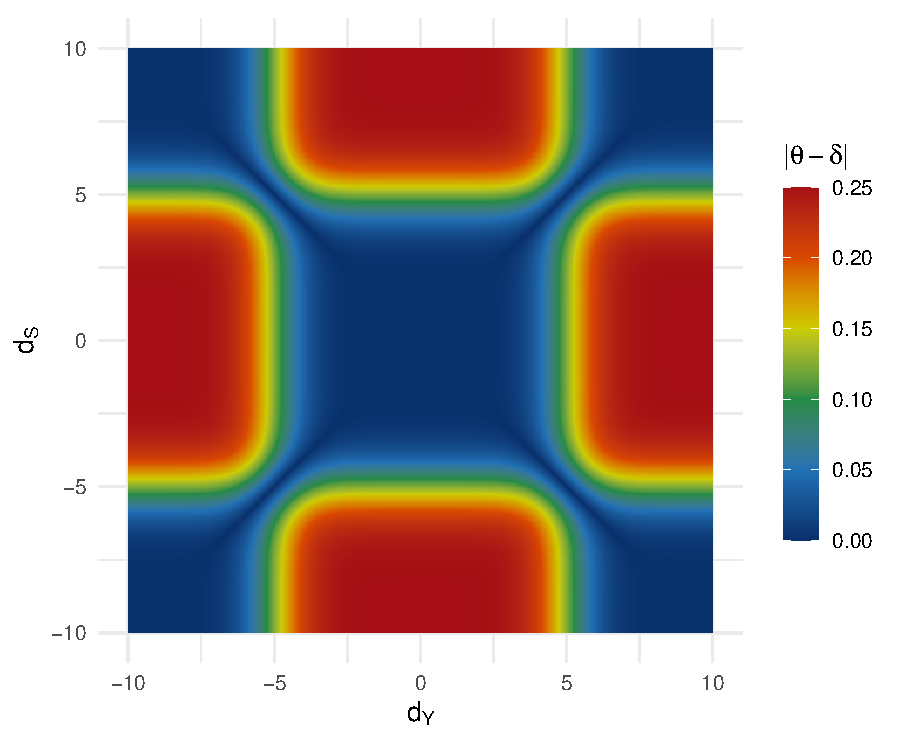
\includegraphics[width=0.8\textwidth]{discrepancy_heatmap.pdf}
    \caption{Plot of the distance \(|\theta - \delta|\) as a function of \(d_Y\) and \(d_S\) in the setting where the distribution of the potential outcomes is Gaussian and its parameters depend on a binary covariate. Here we set \(\Delta = 5\).}
    \label{fig:discrepancy_heatmap}
\end{figure}

This implies that
\begin{align}
    \sup_{d_{Y}, d_{S}} \{ |\theta - \delta| \} = \frac{1}{4} | 1 - 2 \Phi (\Delta)| \Rightarrow \sup_{d_{Y}, d_{S}, \Delta} \{ |\theta - \delta| \} = \frac{1}{4},
\end{align}
where the first supremum is proved analytically in Appendix~\ref{app:binary_covariate_derivation}, and the second follows from the principle of iterated suprema \citep{rudin1976principles}. In particular, \(\theta = 0\) while \(|\delta|\) can be as large as \(\frac{1}{4}\), so even though \(S\) is a perfect surrogate for \(Y\), \(\delta\) may be substantially different from \(0\), while \(\theta\) correctly reflects surrogate validity.

%To understand the intuition behind this result, consider the setting where \(d_{Y} = 0\) and \(d_{S} >> \Delta\). In this case, we have that
%\begin{itemize}
%    \item \(U^{00}_{Y} = \Phi (\Delta)\) and \(U^{00}_{S} = \Phi (\Delta)\), therefore \(\delta^{00} = \Phi (\Delta) - \Phi (\Delta) = 0\),
%    \item \(U^{11}_{Y} = \Phi (\Delta)\) and \(U^{11}_{S} = \Phi (\Delta)\), therefore \(\delta^{11} = \Phi (\Delta) - \Phi (\Delta) = 0\),
%    \item \(U^{01}_{Y} = \Phi (\Delta)\) and \(U^{01}_{S} \approx 1\), therefore \(\delta^{01} \approx \Phi (\Delta) - 1 \),
%    \item \(U^{10}_{Y} = \Phi (\Delta)\) and \(U^{10}_{S} \approx 0\), therefore \(\delta^{10} \approx \Phi (\Delta) - 0 = \Phi (\Delta)\).
%\end{itemize}

\subsubsection{Gaussian Covariate Setting}
\label{subsec:gaussian_covariate_setting}

Let us now consider a setting where \(f = \mathcal{N}(m,s^2)\) and the mean potential outcomes are linear functions of the covariate:
\begin{align}
    \mu^{x} = x \boldsymbol{\beta} \quad \forall \; x \in \mathbb{R}, \quad \text{where} \quad \boldsymbol{\beta} = (\beta_{Y_{1}}, \beta_{S_{1}}, \beta_{Y_{0}}, \beta_{S_{0}})^{\top}.
\end{align}
As we show in Appendix~\ref{app:continuous_covariate_derivation}, the general formulas for \(\theta\) and \(\delta\) are non-trivial functions of the slope parameter \(\boldsymbol{\beta}\) and the covariate distribution parameters \(m\) and \(s\). Then, to simplify the analysis, let us assume perfect surrogacy by imposing the following assumption:
\begin{align}
    \beta_{Y_{1}} - \beta_{Y_{0}} = \beta_{S_{1}} - \beta_{S_{0}} = \Delta.
\end{align}
This implies that the treatment effect is the same for both \(Y\) and \(S\) across all values of the covariate. Under this assumption, \(\theta = 0\) and therefore \(|\theta - \delta| = |\delta|\), which is given by
\begin{align}
    |\theta - \delta| = \left| \Phi \left( \frac{m \Delta}{\sqrt{1 + s^2 \left( (\beta_{Y_{0}} + \Delta)^2 + \beta_{Y_{0}}^2 \right)}} \right) - \Phi \left( \frac{m \Delta}{\sqrt{1 + s^2 \left( (\beta_{S_{0}} + \Delta)^2 + \beta_{S_{0}}^2 \right)}} \right) \right|.
\end{align}
In particular, for \(m, \Delta \neq 0\), we observe that
\begin{align}
  \sup_{\boldsymbol{\beta},\, \Delta} \{ |\theta - \delta| \} = \left| \Phi\!\left(\frac{m\sqrt{2}}{s}\right) - \frac{1}{2} \right| \nonumber \Rightarrow \sup_{\boldsymbol{\beta},\, \Delta,\, m,\, s} \{ |\theta - \delta| \} = \frac{1}{2},
\end{align}
An analytic proof for the first supremum is given in Appendix~\ref{app:continuous_covariate_derivation}, while the second supremum follows by the principle of iterated suprema \citep{rudin1976principles}, and it is approached when \(|\frac{m}{s}| \gg 0\), which occurs when the Gaussian covariate is highly concentrated away from zero.

This means that in this setting, even though \(S\) is a perfect surrogate for \(Y\), \(\delta\) can be substantially different from \(0\) and its value depends arbitrarily on the distribution of the covariate. In contrast, \(\theta\) correctly captures the surrogate validity by being equal to \(0\).

Both settings above illustrate that the choice of discrepancy parameter is crucial, as different choices can lead to very different conclusions about surrogate validity. The rank-based approach focuses on \(\delta\), which may not capture the causal relationship between \(Y\) and \(S\) even in simple settings. We therefore advocate focusing on \(\theta\) instead.

\section{Proposed Bayesian Imputation-Based Approach}\label{sec:bayesian_approach}

Our methodology treats causal inference as a missing data problem, estimating parameters by recovering unobserved potential outcomes through Bayesian imputation. We leverage observed data to generate the posterior distribution of missing outcomes, creating complete datasets that enable flexible unit-level comparisons using any discrepancy metric. Following Section~\ref{subsec:comparison_parameters}, we operationalize this approach by focusing on
\begin{equation}
  \label{eq:V_definitions}
  \begin{aligned}
    V_{Y} & = \Prob(Y_{1i} > Y_{0i}), \quad V_{S} & = \Prob(S_{1i} > S_{0i}), \quad \theta & = V_{Y} - V_{S}.
  \end{aligned}
\end{equation}
At each iteration, we impute the unobserved potential outcomes (e.g., \(Y_{0i}\) and \(S_{0i}\) for \(Z_{i} = 0\)) from their posterior predictive distribution, as detailed in Algorithm~\ref{alg:Bayesian_imputation}.

\begin{algorithm}[htbp!]
\caption{Bayesian Imputation-Based Approach.}
\label{alg:Bayesian_imputation}
\begin{algorithmic}[1]
\Require Observed data \(\{Y_i, S_i, Z_{i}, X_{i}\}_{i=1}^n\), prior parameters, number of iterations \(T\)
\For{\(t = 1\) to \(T\)}
    \For{\(i = 1\) to \(n\)}
        \If{\(Z_{i} = 1\)}
            \State Sample \(P^{(t)}_{0i} \sim \left[ P_{0i} \mid D_{1:n} \right]\)
        \Else
            \State Sample \(P^{(t)}_{1i} \sim \left[ P_{1i} \mid D_{1:n} \right]\)
        \EndIf
    \EndFor
\EndFor
\end{algorithmic}
\end{algorithm}

Using both the observed and imputed outcomes, we compute the probabilities in Equation~\eqref{eq:V_definitions} via Monte Carlo estimators, and obtain a posterior sample for \(\theta\) by taking their difference. Then, to evaluate $S$ as a surrogate, we use the following hypothesis test on \(\theta\):
\begin{equation}
    \label{eq:hypothesis_test_theta}
    \begin{cases}
        H_{0}: \theta \geq \eta, \\
        H_{1}: \theta < \eta.
    \end{cases}
\end{equation}
where \(\eta\) is a pre-specified threshold for surrogate validation. Following \citet{parast2024rank}, we compute a one-sided credible interval for \(\theta\) using a quantile of the \(T\) posterior draws, after discarding the first \(b\) iterations as burn-in:
\begin{equation}
    \widehat{\theta}_{1 - \alpha}
    = \operatorname{quantile}\!\left( \widehat{\theta}^{(b+1:T)},\, 1 - \alpha \right),
\end{equation}
and we reject the null hypothesis if \(\widehat{\theta}_{1 - \alpha} < \eta\); otherwise, we fail to reject it. Equivalently, this decision rule can be expressed in terms of the posterior probability of surrogate validity: we reject \(H_0\) if and only if \(\Prob(\theta < \eta \mid D_{1:n}) \geq 1 - \alpha\), where
\begin{equation}
    \Prob(\theta < \eta \mid D_{1:n}) \approx \frac{1}{T - b} \sum_{t=b+1}^{T} \one\!\left(\widehat{\theta}^{(t)} < \eta\right).
\end{equation}
While this is not a Bayesian hypothesis test in the strict sense, since it does not rely on Bayes factors, it provides a natural and interpretable decision rule grounded in the posterior distribution of \(\theta\). The hypothesis testing step is summarized in Algorithm~\ref{alg:Bayesian_test}.

\begin{algorithm}[htbp!]
\caption{Bayesian Hypothesis Testing.}
\label{alg:Bayesian_test}
\begin{algorithmic}[1]
\Require Samples \(\left\{P^{(t)}_{1:n}\right\}_{t=1}^T\), burn-in \(b\), surrogate threshold \(\eta\), significance level \(\alpha\)
\For{\(t = 1\) to \(T\)}
    \State \(\widehat{V}_Y^{(t)} \gets \frac{1}{n} \sum_{i=1}^{n} \one \big(Y_{1i}^{(t)} > Y_{0i}^{(t)}\big)\)
    \State \(\widehat{V}_{S}^{(t)} \gets \frac{1}{n} \sum_{i=1}^{n} \one \big(S_{1i}^{(t)} > S_{0i}^{(t)}\big)\)
    \State \(\widehat{\theta}^{(t)} \gets \widehat{V}_Y^{(t)} - \widehat{V}_{S}^{(t)}\)
\EndFor
\State \(\widehat{\theta}_{1-\alpha} \gets \operatorname{quantile}\!\Big(\widehat{\theta}^{(b+1:T)}, 1-\alpha\Big)\)
\If{\(\widehat{\theta}_{1-\alpha} < \eta\)}
    \State \textbf{Reject} \(H_0\)
\Else
    \State \textbf{Fail to reject} \(H_0\)
\EndIf
\end{algorithmic}
\end{algorithm}

The primary challenge of this methodology lies in sampling the unobserved potential outcomes. Clearly, for each unit \(i\), the sampling strategy to draw the missing potential outcomes from their posterior distribution crucially depends on the assumed data-generating mechanism, denoted as \(F_{i}\) in Equation~\eqref{eq:data_generating_process}. Therefore, in the next section, we propose two flexible parametric models that can be used for this sampling step.

\subsection{Parametric Models for the Data Generating Mechanism}\label{subsection:parametric_models}

The first model we consider excludes covariates, and therefore more closely aligns with the setting of \citet{parast2024rank}. Specifically, we define \(F_{i}\) from Equation~\eqref{eq:data_generating_process} as follows:
\begin{equation}
  \label{eq:parametric_model}
  \begin{aligned}
    P_{i} & \iid \; \mathcal{N}_{4}\!\left( \mu , \Sigma \right), \quad i=1,\ldots,n, \\
    \mu & \sim \; \mathcal{N}_{4}(\mu_{0}, \Sigma_{0}), \\
    \Sigma &= \text{diag}(\sigma_{1:4}) \,\Omega\, \text{diag}(\sigma_{1:4}), \\
    \sigma_{k} &\iid \; \text{Half-Normal}(0, s), \quad k = 1,2,3,4, \\
    \Omega & \sim \; \text{LKJ}(\tau),
  \end{aligned}
\end{equation}
where we place a Gaussian prior on the mean vector \(\mu\) and we adopt a separation strategy \citep{barnard2000modeling} for the covariance matrix \(\Sigma\), decomposing it into a correlation matrix \(\Omega\) and a scale vector \(\sigma_{1:4}\). This allows us to specify easily interpretable priors: an LKJ prior \citep{lewandowski2009generating} for the correlation and a half-normal prior for the scale.

However, one of the main advantages of our proposed Bayesian framework is its ability to naturally incorporate baseline covariates into the data-generating mechanism. To illustrate this feature, we consider a second model that introduces covariates through a linear regression structure, specifying \(F_{i}\) from Equation~\eqref{eq:data_generating_process} as follows:
\begin{equation}
  \label{eq:parametric_model_covariates}
  \begin{aligned}
    P_{i} &\overset{\text{ind.}}{\sim}\;
            \mathcal{N}_{4}\!\left( B X_{i} , \Sigma \right), \quad i=1,\ldots,n, \\
    B &= \big[ \beta_{1} \; \beta_{2} \; \beta_{3} \; \beta_{4} \big]^{\top}, \\
    \beta_{k} & \iid \; \mathcal{N}_{d}(\mu_{\beta}, \Sigma_{\beta}), \quad k = 1,2,3,4, \\
    \Sigma &= \text{diag}(\sigma_{1:4}) \,\Omega\, \text{diag}(\sigma_{1:4}), \\
    \sigma_{k} &\iid \; \text{Half-Normal}(0, s), \quad k = 1,2,3,4, \\
    \Omega & \sim \; \text{LKJ}(\tau),
  \end{aligned}
\end{equation}
where we place a Gaussian prior on the regression coefficients in the matrix \(B\) and we adopt the same separation strategy for the covariance matrix \(\Sigma\) as in the first model.

\subsection{Identifiability of \texorpdfstring{\(\theta\)}{theta} and Interpretation of its Posterior}
\label{subsection:identifiability}

Both formulations in Equations~\eqref{eq:parametric_model} and \eqref{eq:parametric_model_covariates} are quite simple and intuitive. However, they are both plagued by a common non-identifiability issue. Specifically, it is a well-known fact in the causal inference literature that the joint distribution of the potential outcomes is not identifiable from the observed data, since only one potential outcome is observed for each unit. This issue is typically referred to as the ``fundamental problem of causal inference'' \citep{holland1986statistics}. Therefore, to understand how this issue manifests in our setting, it is useful to take a closer look at the correlation matrix \(\Omega\) in the two models:
\begin{align}
\label{eq:correlation_matrix}
  \Omega = \begin{bmatrix}
    1 & \textcolor{ForestGreen}{\rho_{Y_{1}S_{1}}} & \textcolor{BrickRed}{\rho_{Y_{1}Y_{0}}} & \textcolor{BurntOrange}{\rho_{Y_{1}S_{0}}} \\
    \textcolor{ForestGreen}{\rho_{Y_{1}S_{1}}} & 1 & \textcolor{BurntOrange}{\rho_{S_{1}Y_{0}}} & \textcolor{BrickRed}{\rho_{S_{1}S_{0}}} \\
    \textcolor{BrickRed}{\rho_{Y_{1}Y_{0}}} & \textcolor{BurntOrange}{\rho_{S_{1}Y_{0}}} & 1 & \textcolor{ForestGreen}{\rho_{Y_{0}S_{0}}} \\
    \textcolor{BurntOrange}{\rho_{Y_{1}S_{0}}}& \textcolor{BrickRed}{\rho_{S_{1}S_{{0}}}} & \textcolor{ForestGreen}{\rho_{Y_{0}S_{0}}}& 1
    \end{bmatrix}.
\end{align}
It is easy to see that the green entries in the correlation matrix from Equation~\eqref{eq:correlation_matrix} are identifiable from the data, since they involve correlations between potential outcomes that are observed together in the data. In contrast, the remaining entries are not identifiable from the data, since they involve correlations between potential outcomes that are never observed together for any unit. Moreover, as we showed in Equation~\eqref{eq:decomposition_theta} for the Gaussian case, the red entries directly affect the computation of \(\theta\), while the orange entries do not.

In principle, one could try to address this non-identifiability issue by imposing further assumptions on the correlation matrix \(\Omega\). For example, one could assume that all the non-identifiable entries are equal to zero, which would imply that the potential outcomes are independent of each other. However, this assumption is quite strong and is likely unreasonable in many applications. But if we are not willing to make such strong assumptions, how can we still make sense of the posterior distribution of \(\theta\) obtained from our Bayesian imputation approach?

Under standard regularity conditions --- specifically, that the prior assigns positive mass to every KL-neighborhood of the truth and that the model is identifiable --- the posterior concentrates around the true parameter value (Schwartz's theorem \citep{schwartz1965bayes}; see Appendix~\ref{app:posterior_consistency} for the formal statement and definition of regularity). Our model satisfies the first condition but fails identifiability, and therefore we cannot guarantee that the posterior of \(\theta\) concentrates around its true value. A characterization of what happens instead is given by \cite{gustafson2010bayesian}:
\begin{theorem}
  Let the true data-generating process be defined as
  \begin{equation}
    D_{i} \iid f_{\phi^{*}}, \quad i = 1, \ldots, n,
  \end{equation}
  where \(D_{i}\) is the observed data for unit \(i\) and \(f_{\phi^{*}}\) is the true distribution of the data, parametrized by \(\phi^{*}\). Let the parameter \(\phi\) be decomposed as follows:
  \begin{equation}
    \phi = (\phi_{I}, \phi_{N}),
  \end{equation}
  where \(\phi_{I}\) is the identifiable part of the parameter and \(\phi_{N}\) is the non-identifiable part of the parameter. Let the Bayesian model be defined as
  \begin{align}
    \begin{split}
      D_{i} \mid \phi & \iid f_{\phi_{I}}, \quad i = 1, \ldots, n, \\
      \phi & \sim \pi,
    \end{split}
  \end{align}
  where \(\pi\) is a prior distribution over the parameter \(\phi\). Then, if the identifiable component of the Bayesian model is regular according to Definition~\ref{def:regularity}, the posterior distribution of \(\phi\) concentrates around the set of values that are compatible with the observed data and the model assumptions as the sample size goes to infinity:
  \begin{equation}
    \pi \left( \phi_{I} \in U_{I} \mid D_{1:n} \right) \overset{P_{\phi^{*}}}{\to} 1,
  \end{equation}
  for every neighborhood \(U_{I}\) of the identifiable component \(\phi_{I}^{*}\), where \(P_{\phi^{*}}\) is the probability measure induced by the true distribution \(f_{\phi^{*}}\). Whereas, the posterior distribution of the non-identifiable component \(\phi_{N}\) will behave as follows:
  \begin{equation}
    \pi \left( \phi_{N} \in U_{N} \mid D_{1:n} \right) \overset{P_{\phi^{*}}}{\to} \pi \left( \phi_{N} \in U_{N} \mid \phi_{I} = \phi_{I}^{*} \right),
  \end{equation}
  for every neighborhood \(U_{N}\) of the non-identifiable component \(\phi_{N}^{*}\), where \(\pi \left( \phi_{N} \in U_{N} \mid \phi_{I} = \phi_{I}^{*} \right)\) is the conditional prior distribution of the non-identifiable component given the identifiable component evaluated at its true value.
\end{theorem}
What this last result tells us is that, even though the posterior distribution of \(\theta\) is not fully identified from the data, there is still a process of Bayesian learning that takes place as the sample size increases, and the posterior distribution of \(\theta\) will concentrate around a set of values that are compatible with the observed data and the model assumptions. Therefore, it is still possible to meaningfully perform inference on \(\theta\) for the purpose of surrogate validation. However, it is important to keep in mind that due to the lack of concentration for the non-identifiable component of the parameter, there is a non-vanishing uncertainty in the posterior distribution of \(\theta\) that persists even in the asymptotic limit. This feature of the proposed Bayesian imputation approach may appear to constitute an inherent limitation. Nevertheless, we argue that the methodology retains merit for at least two reasons.

First, the identifiability issue is not unique to our proposed Bayesian imputation approach, but rather it is a fundamental issue that arises in any approach that relies on the observed data to make inference about the joint distribution of the potential outcomes. Therefore, any method that attempts to assess surrogate validity using the observed data will have to contend with this issue in some form. Then, the non-vanishing uncertainty in the posterior distribution of \(\theta\) can be seen as a reflection of the inherent uncertainty in the problem of surrogate validation. However, since the amount of uncertainty injected by the prior does not disappear even asymptotically, it becomes of crucial importance to choose reasonable priors that reflect our beliefs about the data-generating process. In this regard, given the prior specifications chosen in Equations~\eqref{eq:parametric_model} and \eqref{eq:parametric_model_covariates} and, more specifically, the choice of the prior for the correlation matrix \(\Omega\), unless we have strong prior beliefs about the correlation structure of the potential outcomes, it is reasonable to choose a weakly informative prior, such as an LKJ prior with \(\tau = 1\), which corresponds to a uniform distribution over the space of correlation matrices.

Second, even though our proposed Bayesian imputation approach does not showcase the desirable property of consistency, it still provides useful information about surrogate validity and, most importantly, it may still be preferable to alternative approaches that may not suffer by this non-identifiability issue but are unable to correctly capture the causal relationship between the surrogate and the primary outcome. For example, as we showed in Section~\ref{subsec:limitations}, the discrepancy parameter \(\delta\) used by \citet{parast2024rank} may fail to capture the causal relationship between \(Y\) and \(S\) even in very simple settings, while our approach targets a parameter \(\theta\) that is able to correctly reflect surrogate validity. Hence, this suggests that using our approach can lead to more accurate assessments of surrogate validity than the rank-based approach of \citet{parast2024rank} and especially in small-sample settings where the lack of asymptotic consistency may not be as problematic.

\subsection{Selection Procedure for the Validation Threshold}\label{subsec:alternative_threshold}

We now turn to the challenge of selecting the prespecified threshold used to assess surrogate validity, denoted \(\varepsilon\) by \citet{parast2024rank} and \(\eta\) in Equation~\eqref{eq:hypothesis_test_theta}. As noted by \citet{parast2024rank}, the distribution of \(\widehat{\delta}\) is not fully specified under the null in Equation~\eqref{eq:hypothesis_test_delta}, so choosing the threshold \(\varepsilon\) is not a trivial task. They suggest choosing it to ensure a desired power to detect a treatment effect on \(S\). Here, we outline an alternative procedure for selecting \(\eta\) in Equation~\eqref{eq:hypothesis_test_theta}, similar in spirit but better suited to our Bayesian framework, which relies on a Bayes factor, the standard tool for Bayesian hypothesis testing.

The intuition is that we aim to set \(\eta\) such that when $V_S$ is close to $V_{Y}$ i.e., within \(\eta\), $S$ is a valid replacement of $Y$. To do this, we aim to identify $v_s$, which is defined as the value of \(V_{S}\) that ensures a power of \((1 - \beta)100\%\) for the following hypothesis test:
\begin{equation}
    \label{eq:hypothesis_test_V_S}
    \begin{cases}
        H_{0}: V_{S} = \tfrac{1}{2}, \\
        H_{1}: V_{S} > \tfrac{1}{2}
    \end{cases}
\end{equation}
implemented using a Bayes factor. Let $v_Y$ denote the hypothesized treatment effect on $Y$. One reasonable way to choose $v_Y$ is by using the posterior mean of $V_Y$ obtained from our Bayesian imputation framework. Then $v_{Y} - v_{S}$ reflects how far we are willing to let $v_{S}$ be from $v_{Y}$, while still ensuring a \((1 - \beta)100\%\) power. To this end, the value of \(\eta\) is defined as:
\begin{equation}
    \eta = \max \{ v_{Y} - v_{S}, 0 \}.
\end{equation}
We now describe the details behind obtaining the value $v_s$. To compute a Bayes factor that can be used to conduct the hypothesis test described in Equation~\eqref{eq:hypothesis_test_V_S}, we first need to specify a Bayesian model taking \(V_{S}\) as its unknown parameter:
\begin{equation}
    \begin{aligned}
        n \, \widehat{V}_{S} \mid V_{S} & \sim \text{Binomial}(n, V_{S}), ~~\mbox{and}~~ V_{S} & \sim p(V_{S}),
    \end{aligned}
\end{equation}
\vspace{-1mm} % REMOVE THIS IF NECESSARY
where the prior for \(V_{S}\) is a Beta distribution renormalized on \( \left( \frac{1}{2}, 1 \right)\):
\begin{equation}
    p(V_{S}) = \frac{\text{Beta}(V_{S} \mid a, b)}{\int_{\frac{1}{2}}^{1} \text{Beta}(v \mid a, b) \, dv} \; \forall \; V_{S} \in \left(\tfrac{1}{2}, 1\right),
\end{equation}
with \(a, b > 0\) suitably chosen prior parameters, and \(\widehat{V}_{S} = \frac{1}{n} \sum_{i=1}^{n} \one(S_{1i} > S_{0i})\). Note that \(\widehat{V}_{S}\) cannot be computed directly from the observed data, since \(S_{1i}\) and \(S_{0i}\) are never jointly observed for any unit \(i\). However, as we shall see below, this is not an issue, because the procedure to select \(v_{s}\) only requires the sampling distribution of \(\widehat{V}_{S}\) under the null hypothesis and alternative hypothesis, rather than an observed value for it.

The resulting Bayes factor $BF_n$ is derived and given in closed form in Appendix~\ref{app:BF_derivation}. As usual, we would like to ensure a type I error probability of $\alpha$:
\begin{equation}
    \mathbb{P} (BF_{n} > BF_{n, \alpha} \mid H_0) = \alpha.
\end{equation}
Since $n \, \widehat{V}_{S}$ takes values in $\{0, \ldots, n\}$, $BF_{n}$ has at most $n + 1$ distinct values, so $BF_{n, \alpha}$ can be obtained as the $(1 - \alpha)$-quantile of $BF_{n}$ (see Appendix~\ref{app:BF_derivation} for the closed-form distribution of $BF_{n}$ under $H_0$). %The value of $BF_{n, \alpha}$ depends on $n$, $\alpha$, and the prior parameters $a$, $b$.
Given $BF_{n, \alpha}$, we can define $v_{S}$ as the value such that
\begin{equation}
    \mathbb{P} \left( BF_{n} > BF_{n, \alpha} \mid V_{S} = v_{S} > \frac{1}{2} \right) = 1 - \beta.
    \label{eq:V_S_power}
\end{equation}
It is useful to observe that the map
\begin{equation}
v_{S} \mapsto \mathbb{P} \big( BF_{n} > BF_{n, \alpha} \mid V_S = v_{S} \big)
\end{equation}
is monotone on \(\left(\frac{1}{2}, 1\right)\). Therefore, there exists a unique \(v_{S}\) satisfying Equation~\eqref{eq:V_S_power}. The probability can be evaluated using the same procedure described in Appendix~\ref{app:BF_derivation} for the distribution of \(BF_{n}\) given \(V_S = v_{S}\). Since the function is continuous and monotone, \(v_{S}\) can be obtained using standard numerical root-finding algorithms, such as \texttt{uniroot} in \texttt{R}.

\section{Simulation Study}\label{sec:simulation_study}

We evaluated the performance of our proposed Bayesian imputation-based method against the frequentist rank-based approach of \citet{parast2024rank} in terms of test coverage and power via a simulation study in six settings.

Specifically, in Settings 1 to 4, we replicated the data-generating mechanisms used by \citet{parast2024rank} to facilitate direct comparison. In Settings 1 to 3 the potential outcomes for the primary outcome were generated as Gaussian variables, but in setting 1 the surrogate was designed to be useless, since its potential outcomes were generated independently of the primary outcome, while in settings 2 and 3 the potential outcomes for the surrogate were obtained by applying a linear transformation of the primary outcome, with the addition of Gaussian noise. Moreover, in Setting 2, the surrogate was designed to be perfect, since the noise was negligible, while in Setting 3, the surrogate was designed to be imperfect, since the noise was more substantial. In contrast, in Setting 4 the outcome was generated from a non-Gaussian distribution and the surrogate was generated by applying a non-linear transformation with the addition of non-Gaussian noise. In all of these settings, we implemented the model in Equation~\eqref{eq:parametric_model} without covariates. Given the true data generating mechanism, one would expect our proposed method to work well in Settings 1-3, but possibly not work well in Setting 4.

In Settings 5 and 6, we purposefully aimed to break the frequentist rank-based method and highlight the advantage of our proposed approach based on the model in Equation~\eqref{eq:parametric_model_covariates} with covariates. Setting 5 features a binary baseline covariate, with generating parameters chosen to maximize the discrepancy between \(\delta\) and \(\theta\), which are approximately \(0.25\) and \(0\), respectively. Conditionally on the covariate, the potential outcomes are not identically distributed across units, violating a key assumption of the Mann-Whitney test. In this setting the surrogate is a replica of the primary outcome with the addition of Gaussian noise, with treatment effect homogeneity across the two subpopulations and uncorrelated potential outcomes; therefore, any valid surrogate validation method should correctly identify $S$ as valid. Setting 6 features a Gaussian baseline covariate with potential outcomes following a linear Gaussian model. The conditional treatment effect on $Y$ and $S$ is identical (implying $\theta = 0$), but the marginal rank-based discrepancy $\delta$ is nonzero due to the covariate structure, further illustrating the limitation of rank-based methods in covariate-dependent settings. Full details of all data-generating processes, prior parameters, and MCMC settings are given in Appendix~\ref{app:simulation_details}.

We ran \(500\) simulations for each setting, with a sample size of \(n = 50\). We quantify performance in terms of coverage of the confidence/credible intervals of the true parameter (\(\delta\) for the frequentist method and \(\theta\) for the Bayesian method) and power, by which we mean the proportion of simulation iterations where the method deemed the surrogate to be valid. In Setting $1$, the surrogate is not valid, and thus, this is the Type 1 error rate. 

Results are shown in Table~\ref{tab:coverage_power_comparison}. In Settings \(1\) and \(2\), the rank-based method of \citet{parast2024rank} and the Bayesian imputation-based method perform similarly. In in Setting \(3\),improved performance is observed for the Bayesian method with higher coverage and higher power. As expected, in Setting \(4\), where the data-generating process is non-Gaussian and non-linear, the nonparametric rank-based method outperforms the Bayesian method in terms of power. Settings \(5\) and \(6\) highlight the true strength of our proposed Bayesian imputation-based method, where the frequentist method very rarely identifies the surrogate as valid, while our method correctly recognizes the surrogate as valid in all iterations. This is not surprising, since the data-generating process in Settings \(5\) and \(6\) were purposely designed to illustrate the limitations of the  the rank-based method.  The proposed Bayesian method is able to adjust for the binary covariate in these settings, and correctly capture surrogacy. The results demonstrate the power gains of our proposed methodology, though we also intentionally explore its limitations under model misspecification.

\section{Real Data Application}\label{sec:real_data_application}
We illustrate our proposed method using  data from the Diabetes Control and Complications Trial (DCCT). This trial was a multicenter, randomized, clinical study designed to determine the effect of an intensive treatment protocol directed at maintaining blood glucose concentrations on progression of early vascular complications in patients with Type 1 diabetes, compared to a control group that received usual care \citep{dcct1987diabetes,Lachin2021DCCT,diabetes1993effect}.  Specifically, the intensive therapy was designed to achieve normal blood glucose levels with three or more insulin injections or an insulin pump. Usual care consisted of 1 or 2 insulin injections per day. Our primary outcome of interest was change in hemoglobin A1c (HbA1c) from baseline to 4.5 years years post-randomization, while the surrogate was an earlier measurement of change in HbA1c from baseline to 1.5 years post-randomization.

Our analysis is focused on a small subgroup of high-risk participants, specifically those in the secondary-intervention cohort (with baseline mild-to-moderate retinopathy) with a body mass index over 25.0 with a history of smoking. This resulted in an analytic sample of 47 participants. Figure~\ref{fig:dcct} shows the distribution of the primary outcome and the surrogate by treatment arm. Figure~\ref{fig:dcct_scatter_cdf} illustrates the relationship between the surrogate and the primary outcome and the empirical CDFs, whose horizontal gap directly corresponds to the rank-based quantities \(U_Y\) and \(U_S\).

\begin{figure}[ht]
    \centering
    \begin{subfigure}[b]{0.48\textwidth}
        \centering
        
\includegraphics[width=\textwidth]{DCCT_Y.pdf}
        \caption{Primary outcome}
    \end{subfigure}
    \hfill
    \begin{subfigure}[b]{0.48\textwidth}
        \centering
        
\includegraphics[width=\textwidth]{DCCT_S.pdf}
        \caption{Surrogate}
    \end{subfigure}
    \caption{Diabetes Control and Complications Trial (DCCT) data illustration of the distribution of the primary outcome of interest, change in hemoglobin A1c (HbA1c) from baseline to 4.5 years post-randomization (left panel), and the surrogate, change in HbA1c from baseline to 1.5 years post-randomization (right panel), in the treated and control groups within the high-risk subgroup.}
    \label{fig:dcct}
\end{figure}

\begin{figure}[ht]
    \centering
    \begin{subfigure}[b]{0.48\textwidth}
        \centering
        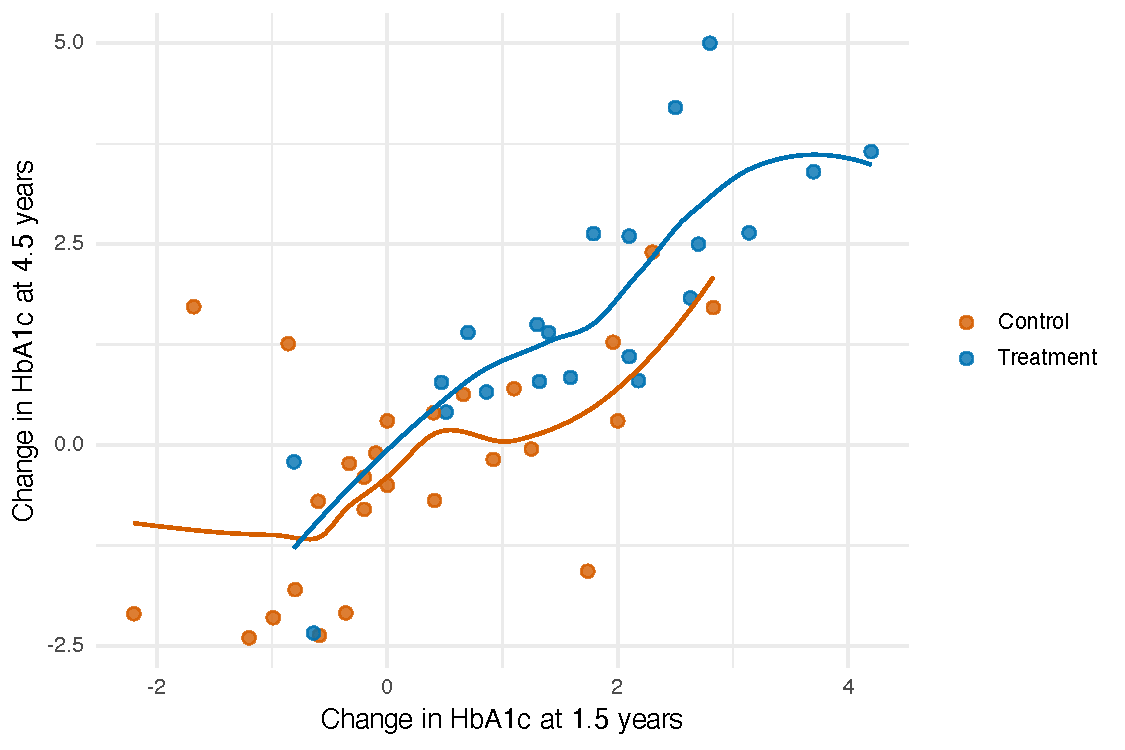
\includegraphics[width=\textwidth]{DCCT_scatterplot.pdf}
        \caption{Surrogate vs.\ primary outcome}
    \end{subfigure}
    \hfill
    \begin{subfigure}[b]{0.48\textwidth}
        \centering
        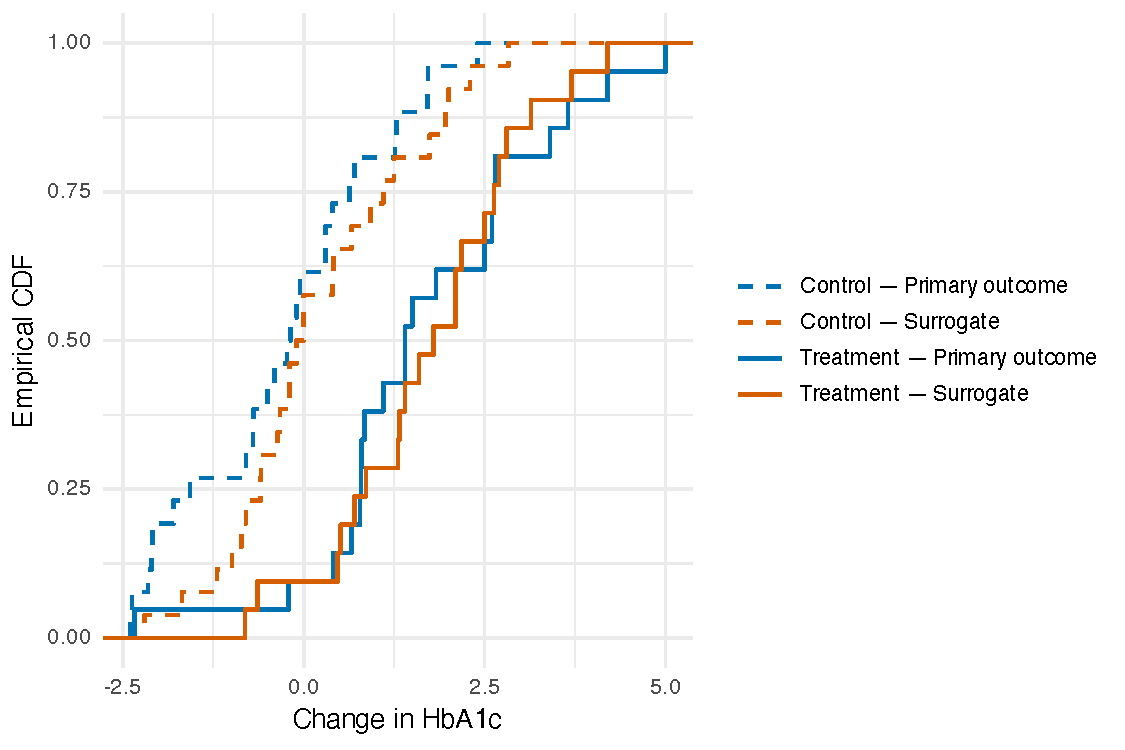
\includegraphics[width=\textwidth]{DCCT_CDF.pdf}
        \caption{Empirical CDFs}
    \end{subfigure}
    \caption{Left panel: scatter plot of the surrogate (change in HbA1c at 1.5 years) against the primary outcome (change in HbA1c at 4.5 years) by treatment arm, with LOESS curves. Right panel: empirical cumulative distribution functions of the primary outcome and the surrogate by treatment arm. The horizontal gap between the solid and dashed curves of the same color reflects the treatment effect on each outcome, directly corresponding to the rank-based quantities $U_Y$ and $U_S$.}
    \label{fig:dcct_scatter_cdf}
\end{figure}

We first applied our proposed method without covariates as described above, with a specified power of 0.70 used to determine the corresponding threshold. The resulting posterior distribution of $\widehat{\theta}$ is shown in the left panel of Figure \ref{fig:dcct_post}, with an average estimate of 0.027, and a credible interval upper bound of 0.149. The calculated threshold was 0.164 and thus, we conclude that change in HbA1c from baseline to 1.5 years is a surrogate for change in HbA1c from baseline to 4.5 years post-randomization. Next, we applied our proposed procedure incorporating the covariates of age (numeric) and sex (male or female). The resulting posterior distribution of $\widehat{\theta}$ incorporating these covariates is shown in the right panel of Figure \ref{fig:dcct_post}, with an average estimate of 0.010, and a credible interval upper bound of 0.149. The calculated threshold was 0.158 and thus, we similarly conclude that this is a valid surrogate. For comparison, the method of \citet{parast2024rank} without covariates (because covariates are not possible to incorporate) resulted in $\widehat{\delta} = 0.044$, a confidence interval upper bound of 0.120, and with a threshold of 0.132, concluding that this is a surrogate marker. While the conclusions are similar, it is certainly worth noting that the estimated difference quantities ($\widehat{\theta}$ vs $\widehat{\delta}$) are smaller using the proposed definition and estimation approaches. Of course, the true values and true surrogacy here are unknown. Nonetheless, this application highlights the potential utility of our proposed approach and, in particular, demonstrates improved characterization of surrogacy and increased efficiency compared to the existing approach.

\begin{figure}[ht]
    \centering
    \begin{subfigure}[b]{0.48\textwidth}
        \centering
        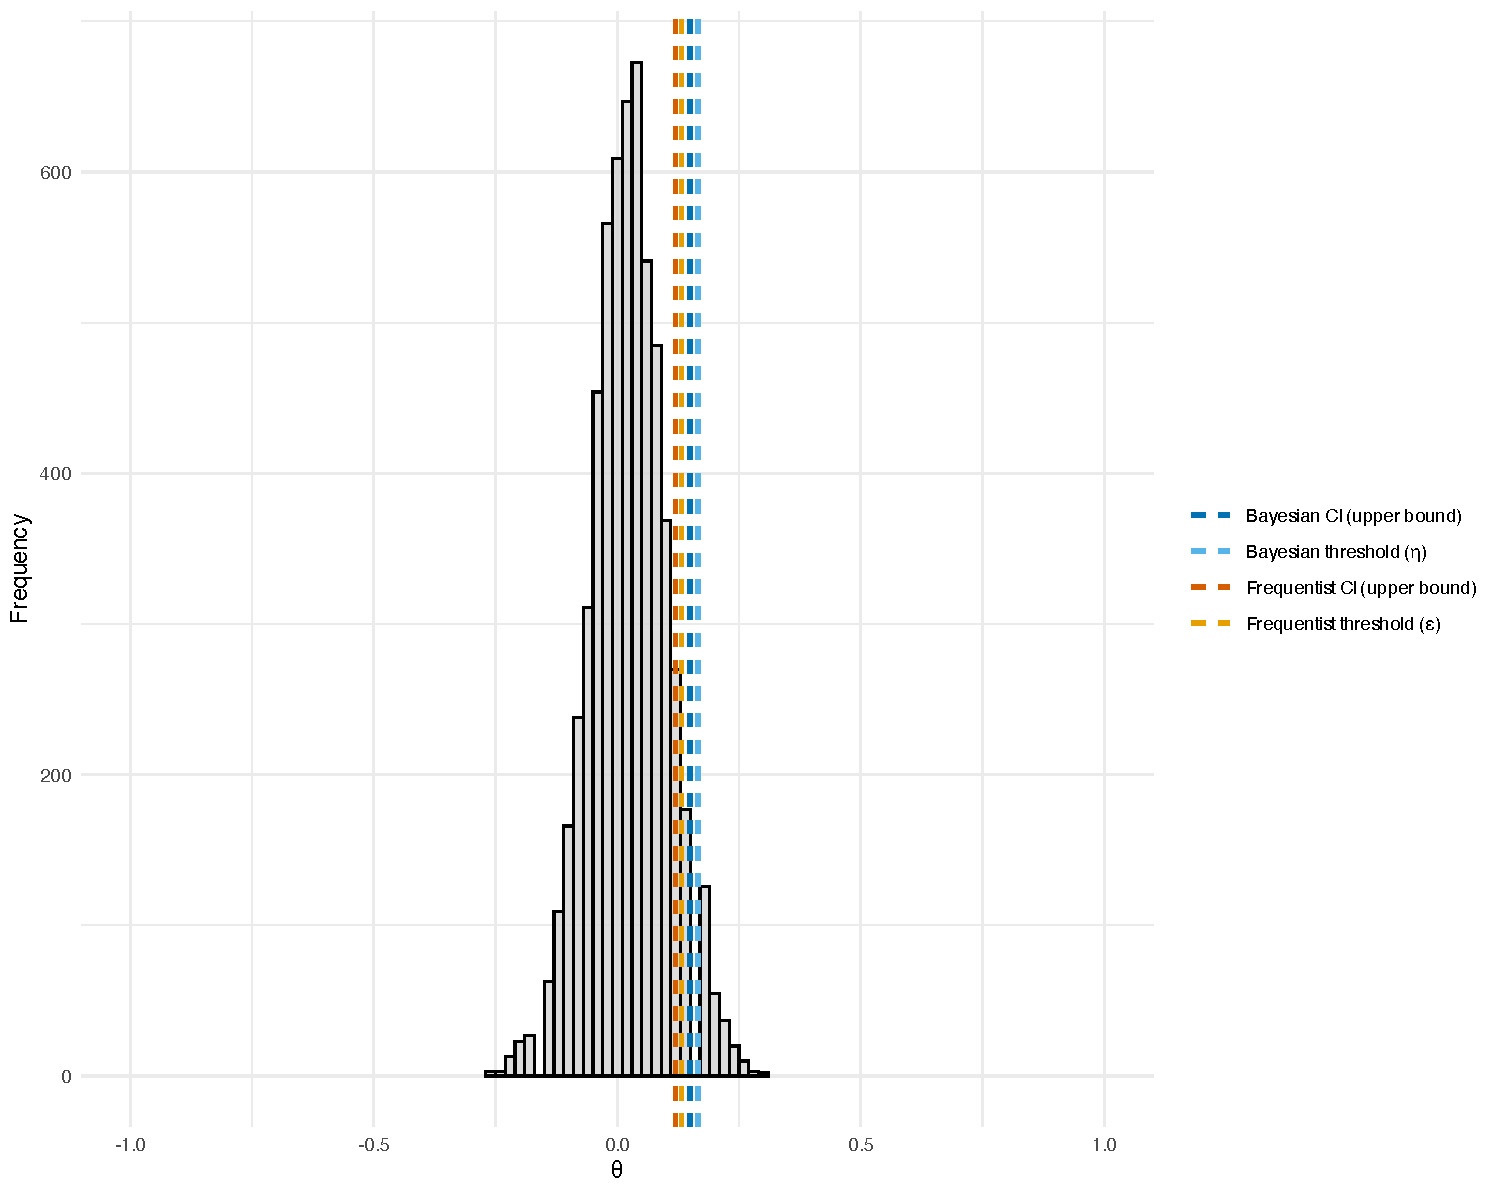
\includegraphics[width=\textwidth]{DCCT_no_X_theta_posterior_plot.pdf}
        \caption{Without covariates}
    \end{subfigure}
    \hfill
    \begin{subfigure}[b]{0.48\textwidth}
        \centering
        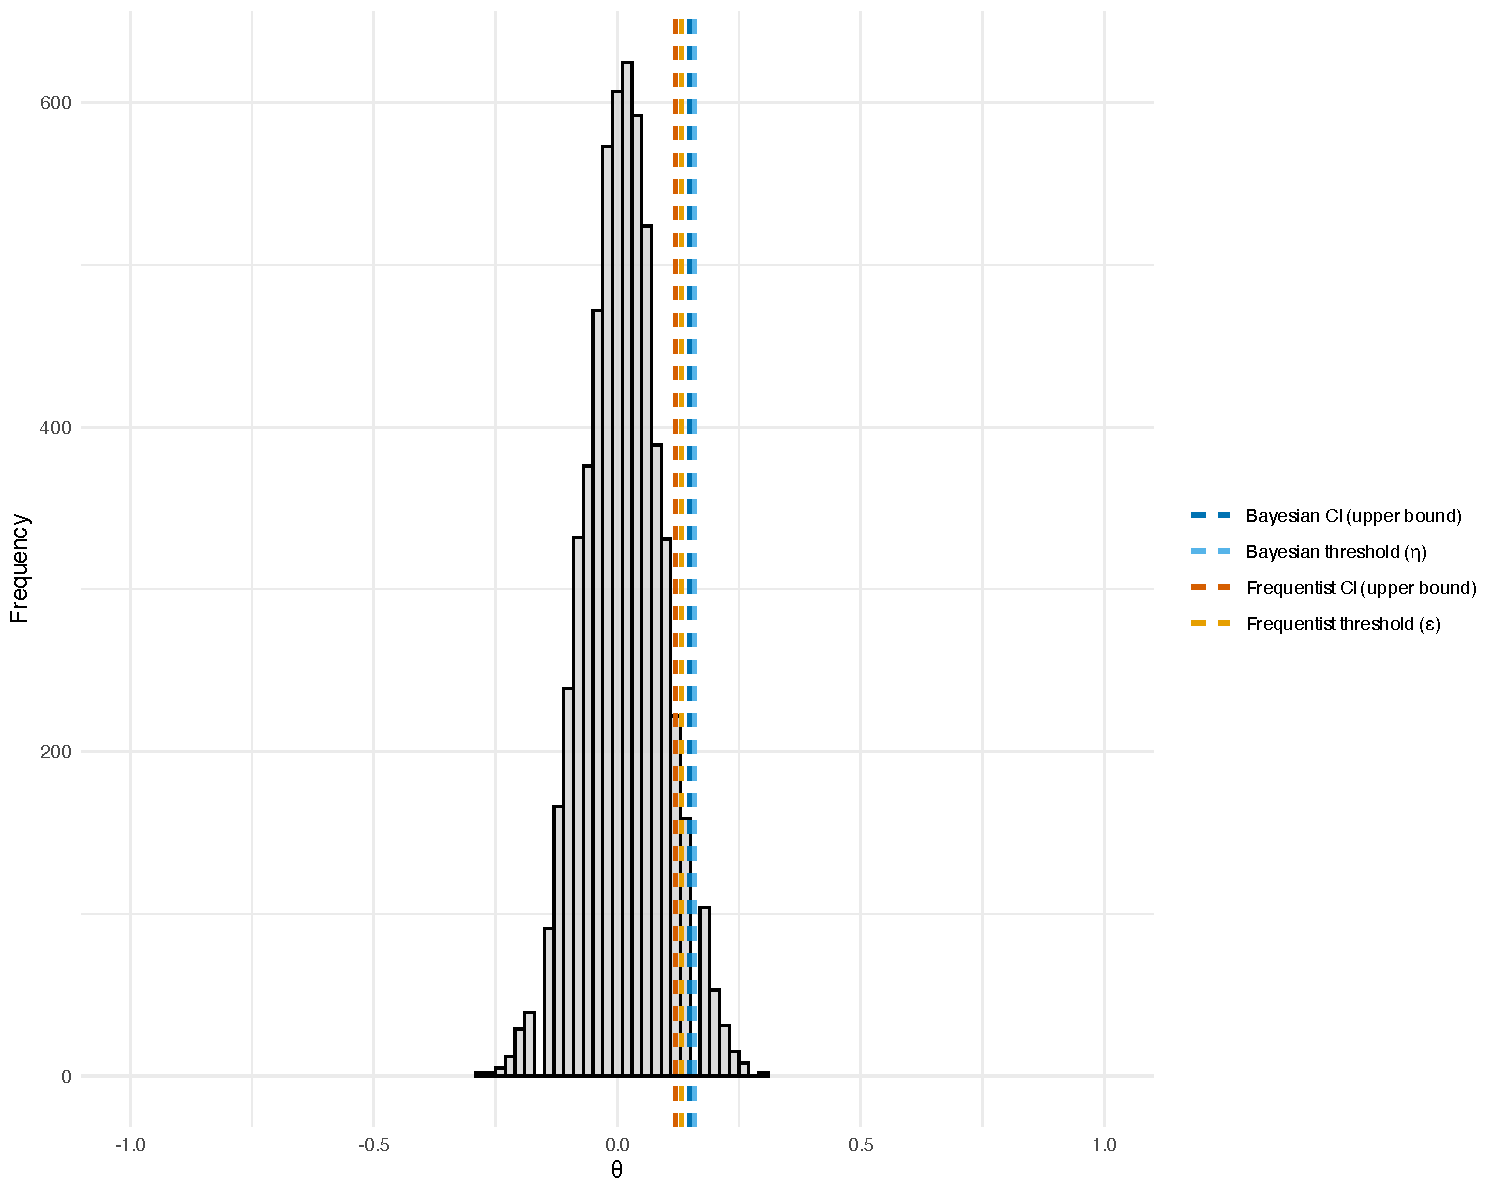
\includegraphics[width=\textwidth]{DCCT_X_theta_posterior_plot.pdf}
        \caption{With covariates (sex and BMI)}
    \end{subfigure}
    \caption{Posterior distributions of $\widehat{\theta}$ when applying the method with no covariates (left panel) and with age and sex (right panel) to the Diabetes Control and Complications Trial (DCCT) data where the primary outcome of interest was change in hemoglobin A1c (HbA1c) from baseline to 4.5 years post-randomization and the surrogate was change in HbA1c from baseline to 1.5 years post-randomization.}
    \label{fig:dcct_post}
\end{figure}

\section{Discussion}\label{sec:discussion}

We proposed a Bayesian imputation framework for surrogate evaluation in randomized clinical trials. Our method overcomes limitations of the frequentist rank-based approach, including lack of causal interpretation, inability to use baseline covariates, and low power, particularly in  in covariate-dependent settings. By imputing unobserved potential outcomes, it enables flexible treatment-control comparisons and inference on surrogate-primary associations. Incorporating baseline covariates improves applicability to complex scenarios, as shown in simulations where our method achieved perfect power versus \(0.075\) for the existing approach. Our proposed methods are implemented in the R package \texttt{BSET} available at \url{https://github.com/PietroCarlotti/BSET}, which also contains all reproducible code.

While our approach overcomes some limitations of the rank-based approach, there is room for further improvement, which we are actively pursuing. A key limitation is the reliance on parametric assumptions about the data-generating mechanism, which are vulnerable to model mis-specification. One possible direction, which we plan for future work, is to relax these assumptions by extending the framework to a Bayesian nonparametric setting \citep{ghosal2017fundamentals}, allowing a data-driven characterization of both the surrogate-outcome relationship and the covariate-outcome association. However, this flexibility comes at a cost of increased computational complexity and larger required sample sizes \citep{miller2018mixture}. Finally, sensitivity analyses examining robustness of our conclusions %regarding surrogate validity
to unidentified covariance parameters would also be useful, and we aim to incorporate such results into our framework and future software.

\section*{Funding and Acknowledgments}
This work was supported by NIDDK grant R01DK118354 (PI:Parast) and [Pietro add funding..?].

The Diabetes Control and Complications Trial (DCCT) and its follow-up the Epidemiology of Diabetes Interventions and Complications (EDIC) study were conducted by the DCCT/EDIC Research Group and supported by National Institutes of Health (NIH) grants and contracts and by the General Clinical Research Center Program (GCRC), the National Center for Research Resources (NCRR). The resources from the DCCT/EDIC study were supplied by NIDDK Central Repository (NIDDK-CR). This manuscript was not prepared under the auspices of the DCCT/EDIC study and does not represent analyses or conclusions of the DCCT/EDIC study group, NIDDK-CR, or NIH.

\bibliographystyle{biom}
\bibliography{BSET_references}

\begin{longtable}[]{@{}cccccc@{}}
\caption{Simulation results comparing the frequentist rank-based method and the proposed 
Bayesian imputation-based method in terms of coverage and power in Settings 1--5, summarized 
over 500 replications with $n=50$ per replication. Bolding indicates the better performing method.}
\label{tab:coverage_power_comparison} \\
\toprule
\textbf{Setting} & \textbf{Valid Surrogate} & \multicolumn{2}{c}{\textbf{Coverage}} & \multicolumn{2}{c}{\textbf{Power}} \\
\cmidrule(lr){3-4} \cmidrule(lr){5-6}
& & Frequentist & Bayesian & Frequentist & Bayesian \\
\midrule
\endfirsthead
\multicolumn{6}{l}{\textit{(continued)}} \\
\toprule
\textbf{Setting} & \textbf{Valid Surrogate} & \multicolumn{2}{c}{\textbf{Coverage}} & \multicolumn{2}{c}{\textbf{Power}} \\
\cmidrule(lr){3-4} \cmidrule(lr){5-6}
& & Frequentist & Bayesian & Frequentist & Bayesian \\
\midrule
\endhead
\midrule
\multicolumn{6}{r}{\textit{(continued on next page)}} \\
\endfoot
\bottomrule
\endlastfoot
1  & No & 0.98 & \textbf{1.00} & 0.00 & 0.00 \\
2  & Yes & 0.98 & \textbf{1.00} & 1.00 & 1.00 \\
3 & Yes & 0.90 & \textbf{0.98} & 0.54 & \textbf{0.64} \\
4 (Misspecified) & Yes & 0.96 & \textbf{1.00} & \textbf{0.56} & 0.06 \\
5 (Binary Covariate) & Yes & 0.925 & \textbf{0.975} & 0.075 & \textbf{1.00} \\
6 (Gaussian Covariate) & Yes & & & & \\
\end{longtable}

\end{document}
